\section{Design}
\label{sec:design}

In this section we will first present the internal structure of the application (in {\sc subsection}~\ref{ssec:struct}) and then we will introduce Beerculator's user interface (in {\sc subsection}~\ref{ssec:ui}).

\subsection{Program structure}
\label{ssec:struct}

Beerculator's implementation is organized in three main elements that are described in the next paragraphs.\\

{\bf Databases} \\ 
There are three tables in the project, which are the following ones:

\begin{itemize}[noitemsep]
\item drinks: contains all the predefined drinks that the user can select;
\item drink\_records: contains the drinks selected by the current user;
\item users: contains all informations about the different users.
\end{itemize}

We also needed queries to fill the \guillemotleft{} drinks \guillemotright{} database, they are all written in a SQL script called list\_drinks.sql.\\

{\bf Java} \\
The project consists in three main classes, Drink.java, DrinkRecord.java and User.java. Their respective UML representations are given by {\sc figures} \ref{fig:drinkJava}, \ref{fig:drinkRecordJava} and \ref{fig:userJava}.\\

The calculation methods, calculateBAC() and hoursUntilSober(double), are implemented in User.java. They are based on the formulas previously introduced in {\sc section}~\ref{sec:spec}. 

\begin{figure}[H]
\centering
   \includegraphics{./figures/drink.png}
   \caption{Class Drink.java, its attributes and its methods}
   \label{fig:drinkJava}
\end{figure}

\begin{figure}[H]
\centering
   \includegraphics{./figures/drinkRecord.png}
   \caption{Class DrinkRecord.java, its attributes and its methods}
   \label{fig:drinkRecordJava}
\end{figure}

\begin{figure}[H]
\centering
   \includegraphics{./figures/user.png}
   \caption{Class User.java, its attributes and its methods}
   \label{fig:userJava}
\end{figure} 

When the user starts Beerculator, the tool sends queries to the database in order to get the predefined drinks. When this is done, the user can interact with the application. He can add drinks, remove some, and enter his personal data (gender and weight). After that, the user can launch the calculation and Beerculator can send him the results. This behaviour is described in an activity diagram, on {\sc figure}~\ref{fig:activ}.

\begin{figure}[H]
\centering
   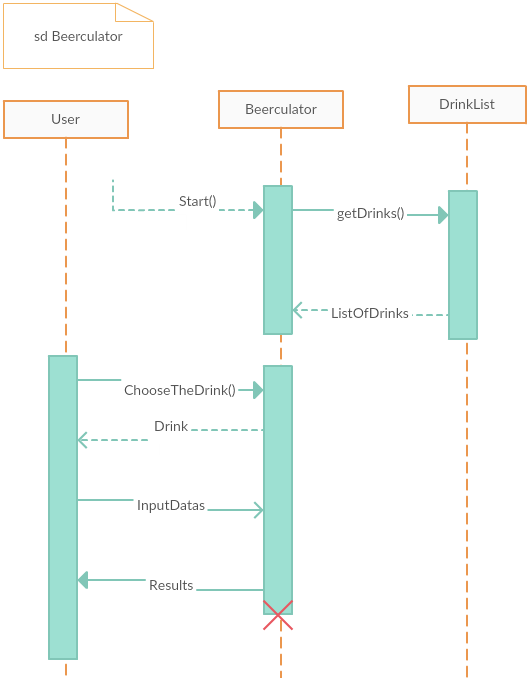
\includegraphics[scale=0.9]{./figures/activDiag.png}
   \caption{Activity diagram for the use of Beerculator}
   \label{fig:activ}
\end{figure}

{\bf Web content}\\
The web content is located in the file Index.xhtml. It is used to generate different URLs based on the session ID. This means that instead of creating a new page for each user, it is just redirected to the page with the right session ID.\\

The web content also includes a folder called WEB-INF, that contains two files: web.xml and faces-config.xml. They are used to manage the server and to handle the Java beans.

\subsection{User interface}
\label{ssec:ui}

Three main elements were needed in Beerculator's interface: one to get the user information (weight, gender, etc), one to display the list of drinks and one to show the results. The user interface can be seen in integrality on {\sc figure}~\ref{fig:ui}. It will also be described tab by tab in {\sc section}~\ref{sec:test}.\\

\begin{figure}[H]
\centering
   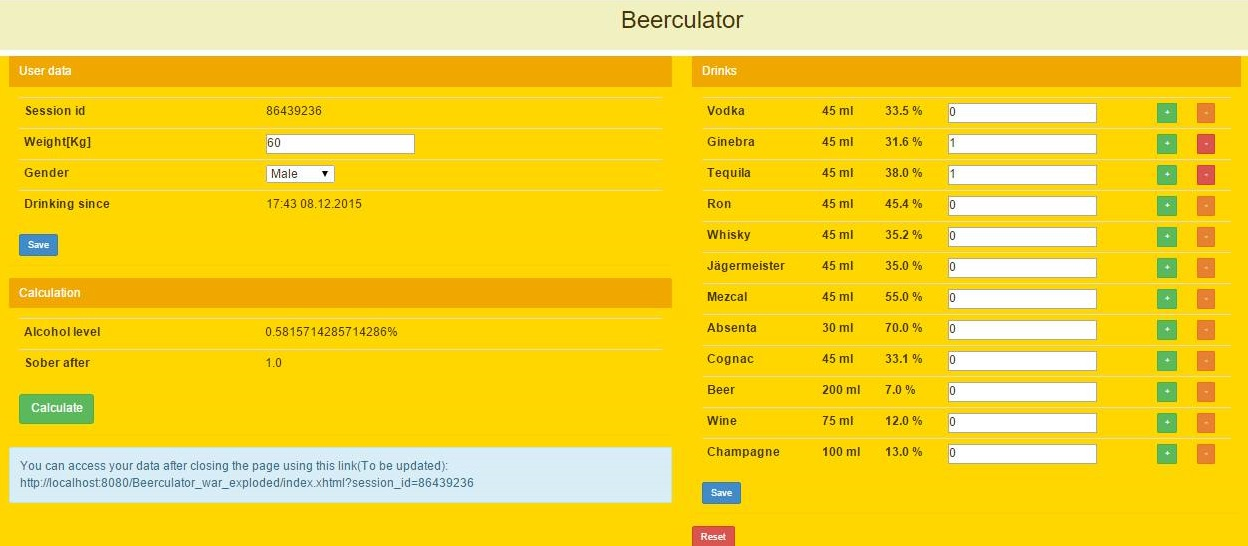
\includegraphics[scale=0.6]{./figures/ui.jpg}
   \caption{User interface of Beerculator}
   \label{fig:ui}
\end{figure}

On the top left part of the interface, the first information is the session ID, that can be used by the user to get back to the page later. Then the user can add all informations that Beerculator needs from him. He can indicate its gender (Male or Female) by picking in a list, and its weight thanks to a text box. Another text box is available for him to tell the time that he started drinking. He can save all those informations, in case he wants to come back later, by clicking on the blue \guillemotleft{} Save \guillemotright{} button.\\

On the right side of the web page, the user can see a list of predefined drinks (with their volume and their alcohol percentage). With each alcohol there are two squares: one green and on red. The user can click on the green one to add one item of the corresponding alcohol to his list of drinks. If he clicks on the red button, one item of this alcohol is removed from the list of drinks. He can also save his list of drinks, for instance if the party is not over and he intends to add some more later, by clicking on the blue \guillemotleft{} Save \guillemotright{} button.\\

When he is done, the user can click on the \guillemotleft{} Calculate \guillemotright{} green button so that Beerculator starts the computation. The results appear on the bottom left corner, in the \guillemotleft{} Calculation \guillemotright{} tab. First the BAC value is indicated, next to label \guillemotleft{} Alcohol level \guillemotright{} , and below it the number of hours until the user gets sober again (next to label \guillemotleft{} Sober after \guillemotright{}).\\

Finally, if the user wants to erase everything and start over, he can press the \guillemotleft{} Reset \guillemotright{} red button on the bottom of the page.
